\subsection{历史背景}
\paragraph{Motivation}互联网的发展, 人们接受的信息越来越多, 从信息稀缺时代逐渐过渡到了信息爆炸时代. 面对数据的海洋, 我们越来越希望我们感兴趣的信息能够直接呈现在我们面前. \tbc{red}{把用户想要的信息推荐给用户} --- 推荐系统的宗旨. 

\paragraph{发展过程}: 
\begin{itemize}
	\item 1994年, 明尼苏达大学GroupLens研究组推出第一个自动化推荐系统GroupLens, 提出将协同过滤作为推荐系统的重要技术
	\item 1995年, 卡耐基梅隆大学的Robert Armstrong等人提出个性化导航系统Web Watcher;斯坦福大学的Marko Balabanovic等人退出了个性化推荐系统LIRA
	\item 1997年, Resnick等人首次提出Recommender System一词
 	\item 1998年, Amazon上线了基于物品的协同过滤算法, 并在千万级用户和百万计商品的规模上进行了应用. Amazon于2003年发表论文\cite{linden2003amazon.com}公布了基于物品的协同过滤算法
	\item 2001年, IBM在其电子商务平台Websphere中增加个性化功能
	\item 2003年, Google开创AdWords盈利模式, 通过用户的广告词来提供相关的广告. 2007年Google为AdWords添加个性化元素, 通过对用户一段时间内的搜索历史进行记录和分析, 以便更精准呈现广告
	\item 2006年, Netflix宣布一项竞赛, 任何人只要能将其现有的电影推荐算法Cinematch的预测准确度提高10\%就能获得100万美金
	\item 2007年, Yahoo提出SmartAds广告方案, 通过分析用户信息以及用户搜索、浏览行为为用户呈现个性化广告
	\item 2007年, 第一届ACM推荐系统大会举行
	\item 2015年, Facebook在其官网公布了其推荐系统原理、性能及使用情况(\href{https://engineering.fb.com/2015/06/02/core-data/recommending-items-to-more-than-a-billion-people/}{Recommending items to more than a billion people}), 相关论文\cite{he2014practical}
	\item 2016年, YouTube发表论文\cite{covington2016deep}介绍Youtube如何向用户推荐个性化的视频
	\item 2016年. , Google发表论文\cite{cheng2016wide}介绍App商店中的推荐系统, 即Wide\&Deep 模型
\end{itemize}

形式上来看, 推荐系统的任务是这样的: 给定一个输入, 从数据集中搜索出一系列数据对象, 并排序后输出. 

输入通常是关于某个用户的表示, 可以是该用户的特征、向量化的表征等, 除此之外用户的行为数据, 如用户的浏览记录、搜索记录、与商品的交互数据、用户的一些动态变化的数据等都可以与用户特征一起作为输入, 而待搜索的数据集中通常是商品的数据, 如商品的特征等, 基于以上丰富的信息, 将输入的信息与数据集中对象进行匹配, 给出推荐的顺序. 

乍一看, 这和搜索很像. 其实这么说也没错, 都是一个\tbc{red}{Learning To Rank}的任务. 其实很多领域研究的问题都很相似, 通过进一步的抽象可以看作是同一个问题. 但随着研究的深入, 为了在一个问题上取得更好的效果, 会相应地结合该领域地特点, 如领域内特有的信息、领域内特有的数据形式等. 因此, 虽然问题之间有重叠, 但为了做得更好, 除了基础的方法, 还需要更深入地挖掘领域地特点!例如, 在推荐系统中, 用户的需求和兴趣是隐含的(隐含在历史数据中, 可能用户都不知道自己喜欢什么), 而搜索中搜索语句是显式的(用户需求是明确的). 

\paragraph{推荐系统主要元素}
\begin{itemize}
	\item 物品集合: 被推荐的物品或内容
	\item 用户: 用户的基本信息, 如基本信息、行为信息、兴趣爱好等
	\item 场景: 用户所处的环境, 如网络环境、所处位置等
	\item 推荐引擎: 根据用户对物品的偏好与用户的画像数据进行拟合, 学习什么样的用户会喜欢什么样的物品. 引擎包含以下重要模块: 
	\begin{itemize}
		\item 召回模块: 根据用户和场景特征, 从整个物品数据集(上百万物品)中挑选用户可能感兴趣的物品, \textbf{挑选出一个较小的候选集}(几百至几千). 召回模块中, 通常使用简单的特征进行快速查询, 比如用户最近点击的物品的相似物品、根据用户兴趣召回物品等. 常用的算法: Word2vec、LDA、LSTM、ItemCF、UserCF、DNN等
		\item 排序模块: 针对召回模块找到的\textbf{候选集进行精排}, 得到用户对候选物品集的评分. 常用的算法: LR、FM、XGBoost、GBDT+LR、Wide\&Deep、FNN、PNN、DeepFM、NFM、DIN等
		\item 后排模块: 得到用户对候选集的评分后, 可以根据一些规则对排序进行调整, 如运营干预、优先级调权等
	\end{itemize}
	\item 推荐结果集: 推荐结果, 或推荐结果的有序排列
\end{itemize}

\subsection{会话推荐}
会话推荐 (session-based recommendation) 是预测用户在一条交互序列中可能会喜欢的下一个商品. 基于深度学习的会话推荐方法试图从用户的历史交互序列中学习和理解用户的行为, 建模用户的偏好. Session-based Recommender System (SBRS) 是指在用户未登录状态下, 仅仅依赖匿名会话进行用户下一个行为预测的一种算法, 在许多领域(如电商、短视频、直播等)有着重要的作用. SBRS 从用户与系统交互过程中的会话来学习用户的偏好. 每一个会话由一段连续的时间内用户与物品的若干个交互组成, 例如在一次网购中所购买的商品.

近期 SBRS 的 SOTA 结果都是基于神经网络模型取得的. 
\begin{myitemize}
	\item 2016年提出的 GRU4Rec 是该系列中经典的一篇, 首次利用RNN对session序列建模, 相比传统的 KNN 和矩阵分解, 效果有明显的提升. GRU4Rec 的核心思想是在一个 session 中, 用户点击一系列 item 的行为看做一个序列, 用来训练 RNN 模型. 预测阶段, 给定已知的点击序列作为输入, 预测下一个可能点击的 item.;
	
	\item 在 GRU4Rec 的基础上, NARM 将注意力机制应用于对 session 的顺序行为及主要意图进行分别建模. 和以往方法不同的是显示地对用户在 session 目的进行建模;
	
	\item 与 NARM 相似, STAMP 利用简单的多层感知机和注意力网络对 session 内长短期兴趣分别表征. STAMP 设计了不同结构分别对 session 内长期兴趣和短期兴趣建模, 取序列中最后一个交互的item表征短期兴趣;
	
	\item 之前序列模型都仅对连续交互相邻 item 之间的序列过渡关系进行挖掘, 而忽略了不相邻 item 之间复杂地转变, SR-GNN 通过引入 GNN 来对 session graph 进行建模, 以此发掘序列内 item 之间复杂的过渡模式;
	
	\item 之前的方法通常忽略了 session 间的关系, GCE-GNN 提出了一种全局上下文增强(global-context enhanced)的 GNN 网络. 能够从两种层次来学习物品的表征, 包括 global-level: 从所有 session 构成的图上进行全局的表征;以及 session-level: 从单个 session 局部 item 转移图上进行局部的表征. 最后融合二者, 并通过注意力机制形成最终的序列表征, 用于序列推荐任务.
\end{myitemize}

\subsection{共现矩阵}
显然, 共现矩阵是一种矩阵, \textbf{关键是它描述了一种什么事实}?$M, N(|M| = m, |N| = 2)$表示两个相同或者不同的集合, 共现矩阵可以用于表达两个集合笛卡尔乘积的元素对的某种关系, $(m_i, n_j)$间的这种关系可以用共现矩阵的元素$CM_{ij}$表示. 

在具体的应用场景中, 
\begin{itemize}
	\item 推荐系统: $M$表示用户集, $N$表示商品集, $CM_{ij}$表示用户$m_i$对$n_j$的喜爱程度(如评分)、是否点赞、是否分享等
	\item 自然语言处理: $M = N$表示词汇表, $CM_{ij}$表示词$m_i$与词$m_j$出现在同一个句子中的次数
	\item 社交网络: $M=N$表示作者集合, $CM_{ij}$表示$m_i$与$m_j$间存在某种关系, 如朋友关系、合作关系等
\end{itemize}
共现矩阵是两个集合的元素间关系的一个很直白的表达. 正是因为直白, 共现矩阵通常很稀疏, 空间需求大. 

\subsection{召回方法分类}
召回即从海量的数据集中找出尽可能包含真实结果的候选集. 常见的分类: 
\begin{itemize}
	\item 行为相似召回: 通过用户与物品的交互行为, 发现行为指向的物品的相似物品
	\item 相似用户召回: 通过用户画像和用户行为等, 计算用户之间的相似性, 根据相似用户的行为进行召回物品
	\item 内容相似召回: 通过对物品内容进行分析, 得到物品之间的相似性, 根据与用户产生交互的物品来召回
\end{itemize}


\subsection{常用相似度计算方法}
\paragraph{同现相似度}
物品A和物品B的同现相似度: 
$$
w_{A,B} = \frac{|N(A) \cap N(B)|}{|N(A)|}
$$
其中, $A(A), N(B)$分别表示喜欢A和B的用户集合. 但是这种相似度有个问题, 当B是热门物品时, 喜欢A的用户中可能绝大部分也会喜欢B, 那么$w_{A,B}$就会接近于1, 即任何物品与热门物品的相似度都会接近于1. 除此之外, 还有个问题, 这个相似度不是对称的, 即$w_{A,B} \neg w_{B,A}$, 这看起来是有点不合理的, 因此, 其改进如下: 
$$
w_{A,B} = \frac{|N(A) \cap N(B)|}{\sqrt{|N(A)| \cdot |N(B)|}}
$$

\paragraph{欧几里得距离}
众所周知, 欧氏距离是欧氏空间中两点之间的距离. 两个物品A, B的向量表示为$\boldsymbol{V}_A, \boldsymbol{V}_B$, 则欧式距离为: 
$$
d(A, B) = ||\boldsymbol{V}_A - \boldsymbol{V}_B||_2
$$
以欧式距离计算A, B间相似性时可如下计算: 
$$
sim(A, B) = \frac{1}{1 + d(A, B)}
$$
或许还有其他的形式, 例如: 
$$
sim(A, B) = e^{-d(A, B)}
$$

\paragraph{皮尔逊相关系数}
介于-1和1之间, 它度量两个序列(可以是用户对物品的偏好/评分序列)之间的线性相关程度. 它度量数字一起按比例改变的倾向性, 也就是说两个数列中的数字存在一个大致的线性关系. 当该倾向性强时, 相关值趋于1. 当相关性很弱时, 相关值趋于0. 在负相关的情况下一个序列的值很高而另一个序列的值低---相关趋势趋于-1. 

使用皮尔逊相关系数计算用户/物品相似度时, 通常取共现矩阵中的行(用户对各个物品的偏好)或列(各个用户对一个物品的偏好)作为数列来计算皮尔逊相关系数. 两个物品/用户A, B的向量表示为$\boldsymbol{x}, \boldsymbol{y}$, 则皮尔逊相关系数为: 
$$
r_{\boldsymbol{xy}} = \frac{\sum_i (x_i - \bar{x})(y_i - \bar{y})}{\sqrt{\sum_i (x_i - \bar{x})^2} \sqrt{\sum_i (y_i - \bar{y})^2}}
$$
其实, 仔细一看, 皮尔逊相关系数和余弦相似度很像, 对$\boldsymbol{x}, \boldsymbol{y}$进行标准化后再进行余弦相似度计算. 皮尔逊相关系数用于计算相似性时有以下问题: 
\begin{itemize}
	\item 没有考虑序列的长短. 例如两个用户交互的物品的交集可能会比较大或较小, 通常交集较大的情况下更可靠, 但是交集更小时计算出的皮尔逊系数可能会更大
	\item 若序列长度为1时, 根据定义则无法计算皮尔逊系数
	\item 若序列中的值都相同时也无法计算皮尔逊系数, 因为方差为0
\end{itemize}


\paragraph{余弦相似度}
两个物品/用户A, B的向量表示为$\boldsymbol{V}_A, \boldsymbol{V}_B$, 则余弦相似度为: 
$$
sim(A, B) = \frac{\boldsymbol{V}_A \cdot \boldsymbol{V}_B}{||\boldsymbol{V}_A||_2 \times ||\boldsymbol{V}_B||_2}
$$

\paragraph{Jaccard系数}
两个物品/用户A, B的向量表示为$\boldsymbol{V}_A, \boldsymbol{V}_B$, 则Jaccard相似度为: 
$$
sim(A, B) = \frac{\boldsymbol{V}_A \cdot \boldsymbol{V}_B}{||\boldsymbol{V}_A||_2 + ||\boldsymbol{V}_B||_2 - \boldsymbol{V}_A \cdot \boldsymbol{V}_B}
$$


\subsection{推荐中要注意的点}
\begin{myitemize}
	\item 长尾效应: 位于长尾位置的曝光率低的项目产生的利润不低于只销售曝光率高的项目的利润. 注意对长尾物品的推荐效果, 热门物品的推荐较长尾物品更容易, 在评价算法效果时要注意对长尾物品的推荐效果
	\item 用户经常购买的物品并不一定能体现用户的偏好, 如很多人都会经常买卫生纸, 但这并不能体现用户很喜欢卫生纸, 卫生纸作为热门物品反而并不能体现用户的偏好. 不同的物品对用户的偏好的贡献是不一样的 --- \textbf{user-aware}
	\item 使用用户行为数据来预测某个用户对某个物品的评分时, 要注意历史行为中的物品起的作用可能是不同的\cite{he2018nais}. 如预测我会不会买iphone时, 可能与我过去买的是什么手机有关 --- \textbf{target item-aware}
	\item 如何对待用户没有交互过的物品?
\end{myitemize}

\subsection{常用指标}
此处介绍的指标不涉及具体的计算公式, 在不同的场景下有不同的具体定义, 计算自然也相应而变. 
\paragraph{覆盖率}覆盖率用来描述一个推荐系统对长尾内容或商品的发掘能力. 关于覆盖率的定义, 最简单的理解是推荐系统能够推荐出来的物品, 占平台中全部物品的比例. 

\paragraph{多样性}用户的兴趣是非常广泛的, 在一个视频应用中, 用户可能既喜欢看烧脑电影, 也喜欢看动作大片. 那么, 为了满足用户广泛的兴趣, 推荐列表需要能够覆盖用户不同的兴趣领域, 即推荐结果需要具有多样性. 想提升推荐系统的多样性, 就需要在较大的时间跨度上去识别和理解用户的兴趣. 

\paragraph{新颖性}新颖, 指给用户推荐那些他们以前没有听说过的内容或商品, 例如在视频应用中应该尽可能多地向用户推荐他们没有看过的电影. 而考虑到很多用户在某个应用中的使用粘性可能并不高, 例如一个用户可能同时是多个视频应用的用户, 所以仅仅依靠用户在自己系统中的行为记录来保证推荐的新颖性是不够的. 

除此之外比较简单方法是基于内容或商品的平均流行度去进行推荐, 因为越不热门的东西越可能让用户觉得新颖. 

不过, 向用户推荐不流行的内容或商品, 其实是牺牲了一定的推荐精度的, 所以我们需要权衡该指标与其它指标之间的平衡——这不仅在于技术层面的考量, 可能也在于商业层面的考量. 

\paragraph{惊喜度}如果推荐结果和用户的历史兴趣不相似, 但却能够让用户觉得满意, 那么就可以说推荐结果的惊喜度很高. 想要兼顾推荐系统的惊喜度并不是一件容易的事情, 因为这意味着需要降低推荐结果和用户历史兴趣的相似度, 所以可能会对预测准确度带来一定的挑战. 

但毫无疑问, 用户需要惊喜, 这会极大提升用户的满意度和使用体验, 所以推荐系统对惊喜度的追求只会不断提高, 且还需要在不影响预测准确度的前提下来实现. 过于关注准确率会导致推荐结果的惊喜度不高. 



\subsection{用户画像}

\subsection{电商推荐}

\subsection{冷启动}
冷启动一般是指缺少有价值的数据, 不利于做个性化的推荐. 主要两种情况: 用户冷启动, 物品冷启动. 

\subsubsection{用户冷启动}

即新来的用户或者交互信息很少的用户. 

\subsubsection{物品冷启动}

即新增的物品或者长尾物品. 

\subsection{负采样}
真实场景下, 数据集并不是现成的, 通常是需要我们自己去挖掘, 去构造数据集的. 在构造数据集之前, 通常需要对真实问题建模, 建模之后我们才知道自己需要什么样的数据集. 在推荐系统中, 拿到的原始数据通常是用户的行为数据, 比如用户观看的视频, 点击序列. 或者只有用户的正反馈 (负反馈), 如点赞 (点踩), 分享, 收藏等, 这时候我们只能知道用户喜欢 (不喜欢) 什么. 即我们通常只能拿到正样本或者负样本. 一般而言, 缺乏的是负样本. 其实得到负样本并不难, 根据长尾定律, 用户只会喜欢一小撮东西, 其他的东西大多是负样本, 那负样本的构造还是个问题吗? 负采样的难点其实在于如何找到那些\textcolor{red}{\textbf{难负样本}}. 什么叫难负样本? \textit{看起来像是用户会喜欢的东西, 但实际上用户并不喜欢}. 为什么要难负样本呢? 当然是为了让模型学习到更鲁棒的区分能力, 类似于二分类中找到一个更准确的分界面.

\subsubsection{随机负采样}
最基本的负采样算法, 它的思想就是平等地对待采样池内的每一个商品, 按相等的概率进行采样. 其逻辑非常简单, 在效率上有着很大的优势. 同时也避免在采样过程中引入新的偏差, 是一个被广泛使用的采样算法. 

\subsubsection{基于流行度的负采样}
它的思想是以商品流行度作为采样权重对采样池内的商品进行带权采样, 流行度越高的商品越容易被采到. 一个容易跳过的问题是\textcolor{red}{\textbf{流行度的定义}}, 一种常见的定义方式该商品的历史交互次数, 即商品被消费次数越多, 其流行度就越高. 这种算法相比于随机负采样, 就是将均匀分布替换成一个基于流行度的采样分布, 只需要在采样前计算出每个商品的流行度作为采样分布, 然后就按照这个分布进行采样即可, 在开销上没有增加特别多.
 
相比于随机负采样, 按照流行度采样的目的是为了提高所采负例的信息量, 提高采样质量. 例如一个非常流行的商品, 却出现在某个用户的未交互商品集中, 那么这个商品就很大概率是用户不喜欢的商品, 那么通过这个负例就可以很好的学习到用户的喜好; 相反, 一个大家都不喜欢的商品, 将它作为负例进行学习, 其实能够带给模型的信息量就很少了, 很难学习到该用户的个性化特征. 而且, 热门物品出现在正样本中的次数也会主导模型的判断, 因此基于热度采样也能对热门样本进行打压.

该方法也有一定的局限性. 首先, 因为采样分布是提前计算好的, 在模型训练过程中, 采样分布不会变化. 因此那些在训练初期能够提高更高信息量的负例, 在经过多次训练后, 其带来信息量可能会有所下降. 其次, 流行度的引入也可能会引入新的偏差, 因为流行度的计算是全局的, 而在用户中, 不同用户类别之间的兴趣可能是有差异的, 如果所给数据中的用户类别分布不均匀, 就可能导致流行度的定义出现偏差. 因此, 负采样的流行度也可以是针对每个用户而言的, 相当于为每个用户进行负采样.

\subsubsection{曝光未点击作为负样本}
这种通常是针对 top $K$ 推荐而言的, 即给用户一个 $K$ 个物品的有序列表, 那些没有被点击的物品作为负样本. 最终的 top $K$ 一般都是经过排序模型筛选过后的物品, 模型认为用户会喜欢的物品, 因此如果用户反而没有点击, 则说明模型预测的出问题了, 还是很符合难负样本的定义的. 

\subsubsection{inbatch 采样}
训模型时, 我们通常是一个 batch 一个 batch 地喂数据的, 因此对于 batch 内某个用户的负样本, 可以选择 batch 内其他用户的正样本作为负样本. 但是这样会有一个问题: 对于长尾物品不利, 会造成选择偏差.

\subsubsection{基于模型进行负采样}
这种方法的思路就是由模型来决定哪些是负样本. 在模型训练过程中, 利用上一轮的模型对样本进行评分, 选择非正样本中评分较高的作为负样本. 或者, 根据评分来调整采样时的权重. 这个方法也是比较常用的, 但可能会出现\textcolor{red}{\textbf{伪负样本}}的问题: \textbf{未交互与不喜欢并不等价}.

\subsubsection{基于向量}
其实, 从直觉上来看, 难负样本是那些像正样本的负样本. 那么如果定义了样本之间的距离就可以直接更具这个来选择负样本了.

\subsubsection{针对场景设计规则}
即针对业务场景, 人工设计负样本采样的规则. 例如在视频推荐中, 可以选择同类型下用户未点击的, 或者点击但是停留时长很短的.

有一个需要注意的问题: 召回和排序中的负样本是不一样的, 不能把排序中的负样本作为召回的负样本. 为什么呢?
\begin{itemize}
	\item 二者的目标不一样, 排序是对已经经过层层筛选的物品进行排序, 排序面对的是潜在的正样本. 召回是为了尽可能多地找到用户可能会喜欢地物品, 面对的是浩瀚的物品集;
	
	\item 曝光为点击的物品本质上已经是召回认为的正样本了, 如果把这些作为召回的负样本则自相矛盾了(\textcolor{red}{不过能否作为新的找回算法, 训练更准确的召回模型呢?}). 同时, 以曝光为点击作为负样本, 这会使得召回模型只能识别那些高曝光的物品, 而失去对长尾物品的鉴别能力;
	
\end{itemize}

\subsection{特征交叉}
DNN 时代已然到来, 号称拟合一切函数的 DNN 貌似带来了新的问题解决方式 --- 数据, 模型, 学习. DNN 刚开始大行其道时, 其中一个显著的优点就是不用做过多的特征工程, 貌似要抢走工程师们挖掘特征的工作. 不过热潮过后, 特征工程再度进入人们视野, 特别是在某些领域 --- 推荐搜索广告等. 

为什么这几个领域如此重视特征工程呢? 愚见: 这些领域使用的通常是表格类型的, 大多是结构化或者半结构化的数据, 参与预测的实体 (如用户, 商品等) 都含有丰富的属性, 这些信息构建在\textbf{人与物之间的联系, 人的社会行为}之上. 当然, 不可忽略搜推里的数据通常是稀疏且高维的. 总的来说, 其包含的规律信息是我们可预见的. 像 CV,  NLP, Speech 等领域, 虽然大部分的信息也是以人类的行为为基础, 大多也是有迹可循的, 但是其中牵扯到很多的自然界中的信息, 如视觉, 语音这些本来就存在与自然界中的信息, 现在很多的工作可能更多地是去理解这些一直以来存在的信息的载体的本质. 

那么现在的特征交叉的工作有哪些呢?

\subsubsection{人工构造}

特征工程的重要性不言而喻, 早期工程师们根据自己对问题的理解, 人工挖掘特征, 找到对目标变量比较重要的特征组合, 将其与原始特征一齐输入到模型中. 这种方法在现在也还是蛮多见的, 例如 Wide\&Deep, Youtube DNN 中都有人工构造特征的影子. 很显然, 这种方式依赖于对问题深刻的理解, 算是特征交叉里刀耕火种的阶段?

一些缺点: 1) 获得高质量的高阶特征的成本. 不同场景下高质量的特征是不一样的, 需要深厚的领域知识; 2) 特征过多, 难以手工构造; 3) 手工构造的特征泛化不足, 难以覆盖一些抽象的模式.

\subsubsection{GBDT+LR}

树模型对特征进行分裂的特性造就了其特征组合的能力, 来自 Facebook 的 GBDT+LR\cite{he_gbdtlr_2014} 则开启了这一潮流 (至少从公开发表上来看是这样的). 

先看看树模型是怎么做特征组合的. 对于树中的每个结点, 树模型会选择最优的特征及分割点进行分裂, 迭代进行下去生成决策树 --- 相当于对输入空间的一个划分. 从根节点道叶子节点的路径对应着一系列 \mintinline{c}{if-else} 组成的规则 --- 即特征组合. 

基于树模型做特征组合的方式也很简单: 每个样本输入到一棵树中可以得到一个 one-hot 向量, 这个向量既是该样本的一种特征组合方式, 可与原始特征一齐输入到预测模型中. 

特点: 1) 可以在目标变量的指导下自动生成高阶的特征组合; 2) 显然, 生成组合特征需要监督信号; 3) 要调整树模型的参数.

\subsubsection{FM}

FM\cite{steffen_fm_2011} 算是自动做特征交叉的鼻祖? FM 能自动对任意两个特征做交叉:

$$
\sum_{i=1}^n \sum_{j=i+1}^n <\bm{v}_i, \bm{v}_j> x_i x_j
$$

FM 会为每个特征学习一个隐向量, 用隐向量的内积作为组合特征的重要性. 其特点: 1) 能够自动做二阶的特征交叉; 2) 隐向量也能一定程度降低数据稀疏性的影响; 3) 一般只支持两阶交叉, 做更高阶的特征交叉时间复杂度大大增加.

除了 FM, 还有一个 FFM\cite{juan_ffm_2016}, 算是 FM 的升级版吧, 在特征上再加了一层 Field (特征域) 的概念, 即每个特征都属于一个 \textit{field}, 如 "科幻片", "喜剧片" 都属于 "电影类型" 这个 field 中. FFM 也主要用来做二阶特征交叉, 也会为每个特征学习隐向量, 但是 FFM 为每个特征在每个域下学习一个隐向量. 如果有 $f$ 个特征域, $n$ 个特征, 那么隐向量的个数为 $n \cdot f$. 其交叉的形式为:

$$
\sum_{i=1}^n \sum_{j=i+1}^n <\bm{v}_{i, f_j}, \bm{v}_{j, f_i}> x_i x_j
$$

很显然, 在使用 FFM 时需要按域来对特征进行分组, 对于类别特征, 其取值作为特征都属于同一个域, 对于连续特征则可以单独作为一个域. 

FFM 的特点: 1) 其参数要远大于 FM, 时间复杂度也更高, 不能像 FM 那样进行化简 (关于 FFM 空间/时间的优化可以参考微博的双线性 FFM, Bi-FFM); 2) 引入了特征域的概念, 特征进行两两交叉时, 能够体现域之间的相关性, 当然这也需要更多的参数来学习.


相关资料: \href{https://tech.meituan.com/2016/03/03/deep-understanding-of-ffm-principles-and-practices.html}{深入FFM原理与实践}. 

\textcolor{red}{\textbf{其实到这里已经可以看到很多后续工作的影子了 --- 为特征学习 Embedding}}. 

\subsubsection{DCN}

DCN\cite{wang_dcn_2017} 及其升级版 DCN-V2\cite{wang_dcnv2_2021} 由 google 提出来的, 二者都属于泛 Wide\&Deep 类的模型. 泛 Wide\&Deep 类的模型主要变化在于 Wide 部分. DCN 提出了 Cross Network 作为其 wide 部分:

\begin{figure}[h]
	\centering
	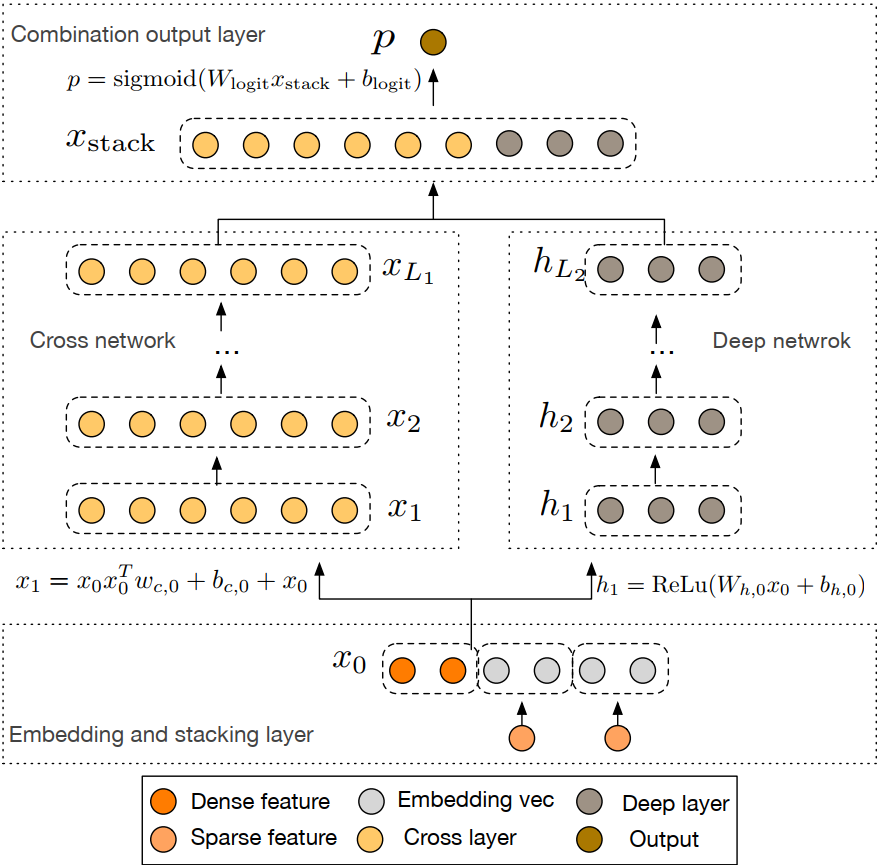
\includegraphics[width=.85\textwidth]{pics/dcn.png}
	\caption{The Deep \& Cross Network}
	\label{fig:dcn}
\end{figure} 

Fig.\ref{fig:dcn} 左边即为 Cross Network. DCN 中的输入由离散特征的 embedding 和 连续特征拼接得到, 然后分别输入到 wide 和 deep 部分, 我们重点关注 wide --- Cross Network 部分. Cross Network 是由 Cross Layer 组成的, 第 $l+1$ 层 Cross Layer 的计算方式:

$$
x_{l+1} = x_0 x_l^T w_l + b_l + x_l = f(x_l, w_l, b_l) + x_l
$$

Cross Network 的第 $l$ 层可以获得 1 至 $l+1$ 阶的特征交叉. 从 DCN 的输入可以看到, 离散特征被替换成了 embedding, 在进行交叉的时候实际是 embedding 的每一位 (及连续特征) 间进行交叉, 并不是以特征为粒度进行交叉的. 

一些缺点: 1) CrossNet 的输出与输入之间存在某种特定形式的关系; 2) CrossNet 的输入是稀疏特征的嵌入, 是 \textit{bit-wise} 方式的特征交叉, 交叉的含义不明显.

DCN-V2 对 DCN 进行了升级. 相比 DCN, DCN-V2 变化主要在 Cross Network. DCN-V2 中 cross layer 的计算方式:

$$
\mathrm{x}_{l+1}=\mathrm{x}_0 \odot\left(W_l \mathrm{x}_l+\mathrm{b}_l\right)+\mathrm{x}_l
$$

其中 $\odot$ 表示逐元素的乘积. 除了 cross layer 的变化, DCN-V2 中 wide 和 deep 部分的结合方式可以是串行的也可以是并行的. 并且为了降低计算开销, 对 cross layer 进行了优化: 将 $W \in \mathbb{R}^{d \times d}$ 变成低秩 (low-rank, 一般认为低秩的矩阵中含有更多信息) 的. DCN-V2 中用两个细长的矩阵来表示 $W = U V^T,\ U, V \in \mathbb{R}^{d \times r}, r \ll \frac{d}{2}$. 因此新的 corss layer 计算方式为:

$$
x_{l+1} = x_0 \odot (U_l (V_l^T x_l) + b_l) + x_l
$$

文中对这种做法给出的一个解释: 在子空间中学习交叉. 因此文中将其与 MMOE 进行结合:

$$
\begin{aligned}
	\mathrm{x}_{l+1} &=\sum_{i=1}^K G_i\left(\mathrm{x}_l\right) E_i\left(\mathrm{x}_l\right)+\mathrm{x}_l \\
	E_i\left(\mathrm{x}_l\right) &=\mathrm{x}_0 \odot\left(U_l^i\left(V_l^{i \top} \mathrm{x}_l\right)+\mathrm{b}_l\right)
\end{aligned}
$$

DCN-V2 的特点: 1) 延续 DCN 的功能, 能以叠加层数的方式获得各阶的特征交叉 (\textit{bit-wise}); 2) 还是 \textit{bit-wise} 粒度的交叉, 不是特征粒度的交叉, 交叉的含义不明确; 3) 增加参数 cross network 的表达能力进行了增强, DCN 中 wide 部分的参数要远小于 deep 部分的参数. 

\subsubsection{xDeepFM}

初看 xDeepFM (eXtreme Deep Factorization Machine)\cite{jianxun_xdeepfm_2018} 感觉写的啥玩意儿, 写的那么复杂, 参数量也要比其他模型高很多, 虽然内心抗拒但还是秉持着完整的心态来写一些吧. xDeepFM 也是泛 Wide\&Deep 类的模型, 相比其他方法, xDeepFM 做的是 \textit{\textbf{vector-wise}} 的特征交叉, 其 wide 部分是 Compressed Interaction Network (CIN). 与其他模型的 wide 部分不同, CIN 的输入是一个矩阵 $\bm{X}^k \in \mathbb{R}^{H_k \times D}$, 输出也是一个矩阵, 矩阵每一行表示一个特征的表征, $\bm{X}^k$ 每一行表示的是一个 $k+1$ 阶的特征.

\begin{figure}[h]
	\centering
	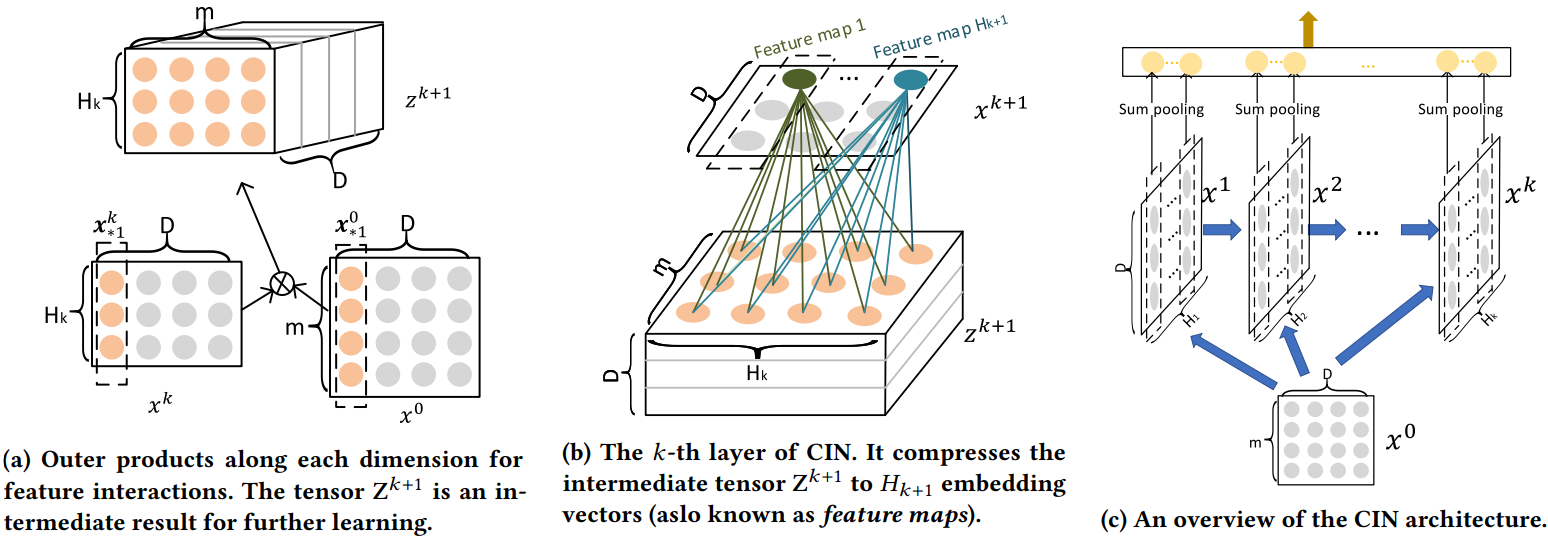
\includegraphics[width=1\textwidth]{pics/cin.png}
	\caption{Components and architecture of the Compressed Interaction Network (CIN).}
	\label{fig:cin}
\end{figure} 

CIN 的计算方式如 Fig.\ref{fig:cin} 所示, 公式为, $\circ$ 表示逐元素乘积:

$$
\mathbf{X}_{h, *}^k=\sum_{i=1}^{H_{k-1}} \sum_{j=1}^m \mathbf{W}_{i j}^{k, h}\left(\mathbf{X}_{i, *}^{k-1} \circ \mathbf{X}_{j, *}^0\right)
$$

结合公式来理解一下 Fig.\ref{fig:cin}. 先通过 $x^k$ 与 $x^0$ 得到 $z^{k+1}$, Fig.\ref{fig:cin}(a) 中的外积, 但其实可以看作是 $x^k$ 的每一行分别与 $x^0$ 的每一行进行逐元素乘积得到张量 $z^{k+1} \in \mathbb{R}^{H_k \times m \times D}$. 所以 $z^{k+1}_{i,j,*}$ 表示一个 \textit{vector-wise} 的交叉, 及 $k+1$ 阶的特征交叉. 因此 $z^{k+1}$ 相当于 $H_k \times m$ 个 $k+1$ 阶的交叉特征, 那这个张量怎么变成一个矩阵呢? 看 Fig.\ref{fig:cin}(b). 结合公式, $x^{k+1}$ 的每一行是通过一个矩阵与 $z^{k+1}$ 计算得到的. 虽然公式看起来复杂, 其实 $x^{k+1}$ 的一行可以看作是 $z^{k+1}$ 中所有 $k+1$ 阶特征的一个线性组合. 由于 CIN 的每一层输出的是 $k$ 阶的交叉特征, 而不是 $1 \sim k$ 阶的交叉特征, 因此需要对 CIN 每层的输出按行进行 \textit{pooling}, 即如 Fig.\ref{fig:cin}(c) 所示, 所有 CIN 层的输出按行进行 \textit{sum pooling} 后进行拼接得到交叉特征. 

需要注意: $H_k$ 是一个超参数, $x^k$ 的每一行都是 $k+1$ 阶的交叉特征, 为什么不直接把 $z^{k+1}$ 按前两个维度展开呢, 这样每个一行都是一个 $k+1$ 阶的交叉特征? 首先, 如果这样做, 那么 $x^k$ 的维度就会一直是 $m^{k+1} \times D$, 这样就相当于一种完全的特征交叉. 显然, 随着层数的加深, 这参数是顶不住的. 因此 CIN 中使用 $H_k$ 个矩阵 $W^{k, h}$ 得到 $H_k$ 种 $k+1$ 阶特征的组合, 起到 \textit{compress} 的作用, 每个 $W^{k, h}$ 相当于一种不同的组合模型. 

xDeepFM 的特点: 1) \textit{vector-wise} 的特征交叉; 2) 参数量大大增加; 3) 每个特征的 embedding 的维度必须相同.

\subsubsection{AutoInt}
AutoInt (Automatic feature Interaction Learning)\cite{song_autoint_2019} 也是一篇看起来很复杂的论文, AutoInt 不是泛 Wide\&Deep 的结构. AutoInt 的目标是给定一个特征向量, 学习特征的低维表示, 其蕴含了高阶的交叉特征. AutoInt 的模型结构如 Fig.\ref{fig:autoint} 所示, 简言之: 通过 \textit{self-attention} 学习每个特征的高阶表示. 所以重点就是 \textit{self-attention}, 如果熟悉这个的话其实就已经知道 AutoInt 是怎么做的了. 

\begin{figure}[h]
	\centering
	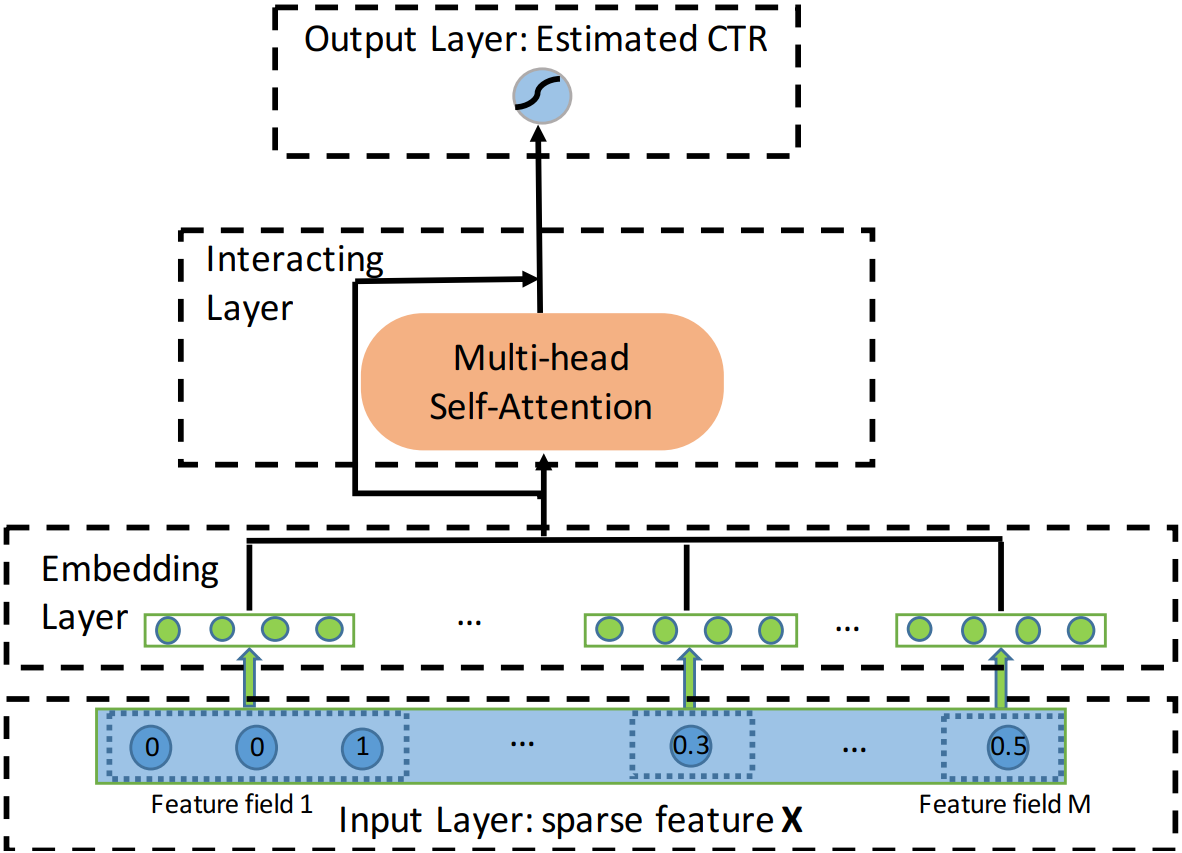
\includegraphics[width=.65\textwidth]{pics/autoint.png}
	\caption{Overview of AutoInt.}
	\label{fig:autoint}
\end{figure} 

AutoInt 中为每个特征 (包括离散特征和连续特征) 学习一个表征. AutoInt 中使用的是多头自注意力 (Multi-head Self-Attention), 并且加了一个残差, head $h$ 的计算方式:

$$
\begin{gathered}
	\alpha_{\mathrm{m}, \mathbf{k}}^{(\mathrm{h})}=\frac{\exp (\psi^{(h)}\left(\mathbf{e}_{\mathrm{m}}, \mathbf{e}_{\mathbf{k}}\right))}{\sum_{l=1}^M \exp (\psi^{(h)}\left(\mathbf{e}_{\mathbf{m}}, \mathbf{e}_{\mathbf{l}}\right))} \\
	\psi^{(h)}(\mathbf{e}_{\mathrm{m}}, \mathbf{e}_{\mathrm{k}})=\langle\mathbf{W}_{\text {Query }}^{(\mathbf{h})} \mathbf{e}_{\mathbf{m}}, \mathbf{W}_{\text {Key }}^{(\mathbf{h})} \mathbf{e}_{\mathbf{k}}\rangle \\
	\widetilde{\mathbf{e}}_{\mathbf{m}}^{(\mathbf{h})}=\sum_{k=1}^M \alpha_{\mathrm{m}, \mathbf{k}}^{(\mathbf{h})}(\mathbf{W}_{\text {Value }}^{(\mathbf{h})} \mathbf{e}_{\mathbf{k}})
\end{gathered}
$$

$\widetilde{\mathbf{e}}_{\mathbf{m}}^{(\mathbf{h})}$ 就是特征 $m$ 经过 head $h$ 的输出, 将多个头的输出进行拼接即是特征 $m$ 经过多头注意力的输出, 再加上残差即可 (残差是不可少的, 类似于 DCN 中的残差, 保证每一层的输出能够得到所有阶数的交叉特征). 注意到, 交叉的阶数随着层数指数增长, 因为自注意力层做特征交叉时是高阶特征与高阶特征交叉, 而不是高阶特征与原始特征交叉. 

AutoInt 的特点: 1) 通过 \textit{self-attention} 机制做特征交叉; 2) 交叉的阶数随层数指数增长; 3) 通过 \textit{attention} 有更好的解释性(其他方法也可以通过类似的方式获得解释性?).